 

\begin{quotation}
  To understand brain function, the focus of [our] investigations must
  expand from detailed responses and structure of single cells to
  include unit responses to the activity of other cells, and how these
  responses are distributed over a population of similar cells as
  wells as across populations of different cells.  - \emph{Shahib Shamma [citation]}
\citet{Shamma:1998}
\end{quotation}

% Modelling in the auditory periphery has benefited extensively from
% the work of Liberman, Greewood, Patterson, Young, Sachs and others,
% in acoustic \texttt{in vivo} experiments.


% =========================================================================

\section{Introduction}

Shihab Shamma calls upon the science community, particularly members
of its physiology and neuroscience subgroups, to investigate the role
of populations of neurons in to pay attention to the role of
populations of neurons in neurophysiology. In this chapter I intend to draw on the wealth of experimental data
accumulated by the auditory neuroscience community to create a
detailed, biophysically-realistic neural network model of the cochlear
nucleus stellate network.  The design and methods for the construction
of the model will provide insights relevant to other neural network
models, especially those that use highly-specific sensory pathways.

Though it remains the case that ``choices, assumptions, and guesses
(are) an integral part of neuronal modeling''
\citep{SegevBurkeEtAl:1998}, there is much to be gained from
biophysically-realistic modeling approaches, especially in the heavily
experimented cochlear nucleus. The developments in computational power
and enhanced experimental techniques in multi-unit recordings are
enabling more detailed neural models. Examples of parameter estimation
and fitting in neural models are also becoming more advanced, for
example NeuroFitter[citation] and MultiRunFitter (a feature in
NEURON).  \yellownote{See further on neural detail in auditory system
  \citep{LuRubioEtAl:2008}}

\medskip{}

\yellownote{Discuss use of Poisson models vs HH-like models.  Discuss
  single cell simulation vs whole network simulation during
  optimisation.}  To develop and optimise detailed neural models and
neural network models, reproducible research methods are required. In
this chapter we use a tabular method, introduced by
\citet{NordlieGewaltigEtAl:2009}, to summarise the model used in each
optimisation step. This method aims to show a consistent and
recognisable format for presenting various neural network models and
their constituents.  The tables consist of A) the model summary, B)
cell type populations, C) connectivity between cell types, D) neuron
and synapse models, and E) optimisation parameters.

\medskip{}

In this chapter, I construct the stellate network of the cochlear
nucleus using a sequential method.  The parameters of each cell type
are fixed based on experimental data or are optimised based solely on
responses to simple stimuli. The network model draws on the following
cells and models:
\begin{itemize}
\item the Carney phenomenological auditory model
  \citet{ZilanyBruceEtAl:2009}: This model provides spiking input to
  cochlear nucleus neurons across frequencies and spontaneous rate
  types of the auditory nerve from an arbitrary input stimulus.  The
  model was adapted to produce fixed responses for high and low SR
  auditory nerve fibres (ANF).
\item the Golgi cell: a GABAergic VCN marginal shell unit that is
  presumed to regulate excitability in the granule cell domain and
  core VCN units \citep{FerragamoGoldingEtAl:1998}.
\item the D-stellate cell: the glycinergic, large multipolar cell with
  onset-chopper PSTH response acts as a co\-incidence detector and
  wide-band inhibitor in the VCN and DCN; and
\item the Tuberculo\-ventral cell: a glycinergic, type-II EIRA unit in
  the deep layer of the DCN.  This cell acts as a delayed
  echo-suppressor and narrow-band inhibitor, with recurrent
  connections between D- and T-stellate cells in the VCN
\item the T-stellate cell: one of the major output projection cells of
  the cochlear nucleus to the inferior colliculus, this multipolar
  neuron has been shown to have robust spectral representation and
  enhanced synchronisation to modulation.
\end{itemize}

\medskip{}

Detailed model requires a good input model, a good neural model and
experimental data with which to fit the parameters.  \yellownote{In
  this para: Connect the introduction section to the Auditory model
  below. Discuss the use of the Carney model in the CN stellate
  model.}


\section{Auditory Model}

Sounds enter the ear and are transformed to neural signals in the
auditory nerve mechanical vibrations in the cochlea by the middle
ear. \yellownote{These sentences need citations.  This paragraph may
  be include in the Lit Review section.}  They are then transformed to
electrical signals in the inner hair cells and then to action
potentials of the auditory nerve fibres. The auditory system is
topographically ordered from the basilar membrane to the cortex in
terms of a frequency selectivity or computed sensory feature map.  The
exceptional feature of hearing perception in animals (i.e. advanced
signal processing and localisation) comes from a one-dimensional input
at the round-window of the cochlea. This processing then enters a
bottle-neck at the auditory nerve, that receive input from the inner
hair cells.


The population of auditory nerve fibers (ANFs) that project to the CN
and retained throughout the auditory pathway
\citep{Lorente:1981}. ANFs bifurcate after entering the cochlear
nucleus to innervate the VCN and DCN, Fig.~\ref{fig:CNdiagram}A. Type
I ANFs are categorised into high spontaneous rate (HSR,
Fig.~\ref{fig:CNdiagram}A solid line) and low spontaneous rate (LSR,
Fig.~\ref{fig:CNdiagram}A dashed line) fibres. LSR fibres have a
higher threshold and do not saturate like HSR fibres. They also
project to the granule cell domain (GCD, Fig.~\ref{fig:CNdiagram}A,
\citep{RyugoParks:2003,RyugoHaenggeliEtAl:2003} along with the
smaller, unmyelinated type II ANFs, which suggests they play a
different role in sound processing to HSR fibres.


\begin{figure}[tbh]
  \begin{center}
%    \includegraphics[keepaspectratio=true]{NoFigure}
    % \resizebox{2.25in}{!}{\includegraphics[width=2.25in,keepaspectratio]{gfx/Cat_Human_CN.jpg}}
    \caption{Cochlear nucleus innervation in Man and Cat }
    \label{fig:CNdiagram}
  \end{center}
\end{figure}


\medskip{}

\yellownote{Discuss auditory model history. Expand reasons for wanting
  to create a biophysically realistic model of the CN. Discuss reason
  for using whole network in TV and TS optimisation} The methods of
modeling in the auditory system over the last 30 years have preferred
the use of simulating one frequency channel to represent a single
neuron's response \citep{DavisVoigt:1991,Carney:1993}.


\yellownote{ a paragraph on the history of AN modelling
  \citep{LeakeSnyderEtAl:1993,ArnesenOsen:1978,CloptonWinfieldEtAl:1974}.
  Perhaps Rose et al 1959 would be better suited here}
%
\medskip{}

In examining the properties of a detailed neural model of the cochlear
nucleus, a realistic and phenomenologically sound auditory model is
needed to represent sounds and transformations that occur in the
central auditory system.

\begin{figure}[tbh]
  \begin{center}
%    \resizebox{3.5in}{!}{\includegraphics[keepaspectratio=true]{NoFigure}}
%    \resizebox{3.5in}{!}{\includegraphics[keepaspectratio=true]{gfx/ZilanyBruceFig}}
    \caption{Auditory periphery model \citep{ZilanyBruceEtAl:2009}}
    \label{fig:ZilanyBruceFig}
  \end{center}
\end{figure}

\yellownote{ a paragraph on the inner working of the AN model}

The auditory nerve inputs to the cochlear nucleus model neurons are
provided by phenomenological auditory periphery models: The ARLO model
\citep{HeinzZhangEtAl:2001}, the Bruce model
\citep{BruceSachsEtAl:2003,ZilanyBruce:2006,ZilanyBruce:2007}, and the
Zilany model \citep{ZilanyBruceEtAl:2009}. The ARLO model consists of
an outer/middle ear pre-processing filter, a cochlear filterbank,
IHC/AN synapse model and dead-time modified Poisson spike
generator. \citep{HeinzZhangEtAl:2001} incorporated cochlear filters
based on the critical bandwidths obtained from psycho\-physical
experiments in humans. The ARLO model of the cat auditory periphery,
with non-linear compression and two-tone suppression, is used in this
study except in the vowel simulation where the human auditory
periphery model is used.

\medskip{}

The \citet{ZilanyBruce:2007} model is enhanced by an additional signal
path and its predictions have matched a wide range of physiological
data in normal and impaired cat data.The current Carney model
comprises an enhanced power-law synapse model, with internal $1/f$
noise, to enhance the behaviour of long-term depencdence in ANFs
\citep{ZilanyBruceEtAl:2009}.

\medskip{}

\yellownote{Make the decision and just refer to the cat model
  throughout} Updating of the Carney auditory model has led to the
change in the model's configuration from an original implementation of
the rat model.  The default species is the cat and will be used in the
data presented in this chapter.

\subsubsection{Physiological Responses}

Analysis of the frequency response area of ANF generates known
parameters for each fibre, these are:
\begin{itemize}
\item the spontaneous rate (SR), generated in silence and is
  categoried into two groups High SR ($>$18 sp/s) and Low SR ($<$ 18
  sp/s);
\item threshold, the sound pressure level(SPL) at which the cell
  responds above the spontaneous rate
\item characteristic frequency (CF)
\end{itemize}

\begin{figure}[tbp]
  \begin{center}
%    \resizebox{3.5in}{!}{\includegraphics[keepaspectratio=true]{NoFigure}}
    % \resizebox{3.5in}{!}{\includegraphics[keepaspectratio=true]{C:/nrnwork/oldwork/ra/TTCsANLSR}}
    % \resizebox{3.5in}{!}{\includegraphics[keepaspectratio=true]{C:/nrnwork/oldwork/ra/TTCsANHSR}}
    \caption{Response areas of low SR and High SR ANFs }
    \label{fig:CochlearTTCs}
  \end{center}
\end{figure}

%% \begin{figure}
%%   \begin{center}
%%     \includegraphics[keepaspectratio=true]{gfx/ClickFB}
%%     \caption{Cochlea Filterbank to click stimuli}
%%     \label{ClickFB}
%%   \end{center}
%% \end{figure}

\begin{figure}[tbh]
  \begin{center}
%    \resizebox{3.5in}{!}{\includegraphics[keepaspectratio=true]{NoFigure}}
%    \resizebox{3.5in}{!}{\includegraphics[keepaspectratio=true]{ClickDelay}}
    \caption{Response of AN and CN cells to click stimuli }
    \label{fig:ClickDelayAN}
  \end{center}
\end{figure}


\section{Cochlear Nucleus Stellate microcircuit}

\subsection{Neural models}
[Discuss R\&M model]

\medskip{}

\subsection{Tonotopic connectivity}

The channels are separated using even spatial distance (based on the
basilar membrane and auditory nerve separation) with centre frequency
calculated by the Greenwood function for the cat
\citep{Greenwood:1990}.

Figure \ref{fig:CNconn} shows the method for Gaussian spread of
connections between cell types in the CN.  The channels are separated
using even spatial distance used for the AN filterbank.


\begin{figure}[tbh]
  \begin{center}
%    \resizebox{3.5in}{!}{\includegraphics[keepaspectratio=true]{NoFigure}}
%    \resizebox{5in}{!}{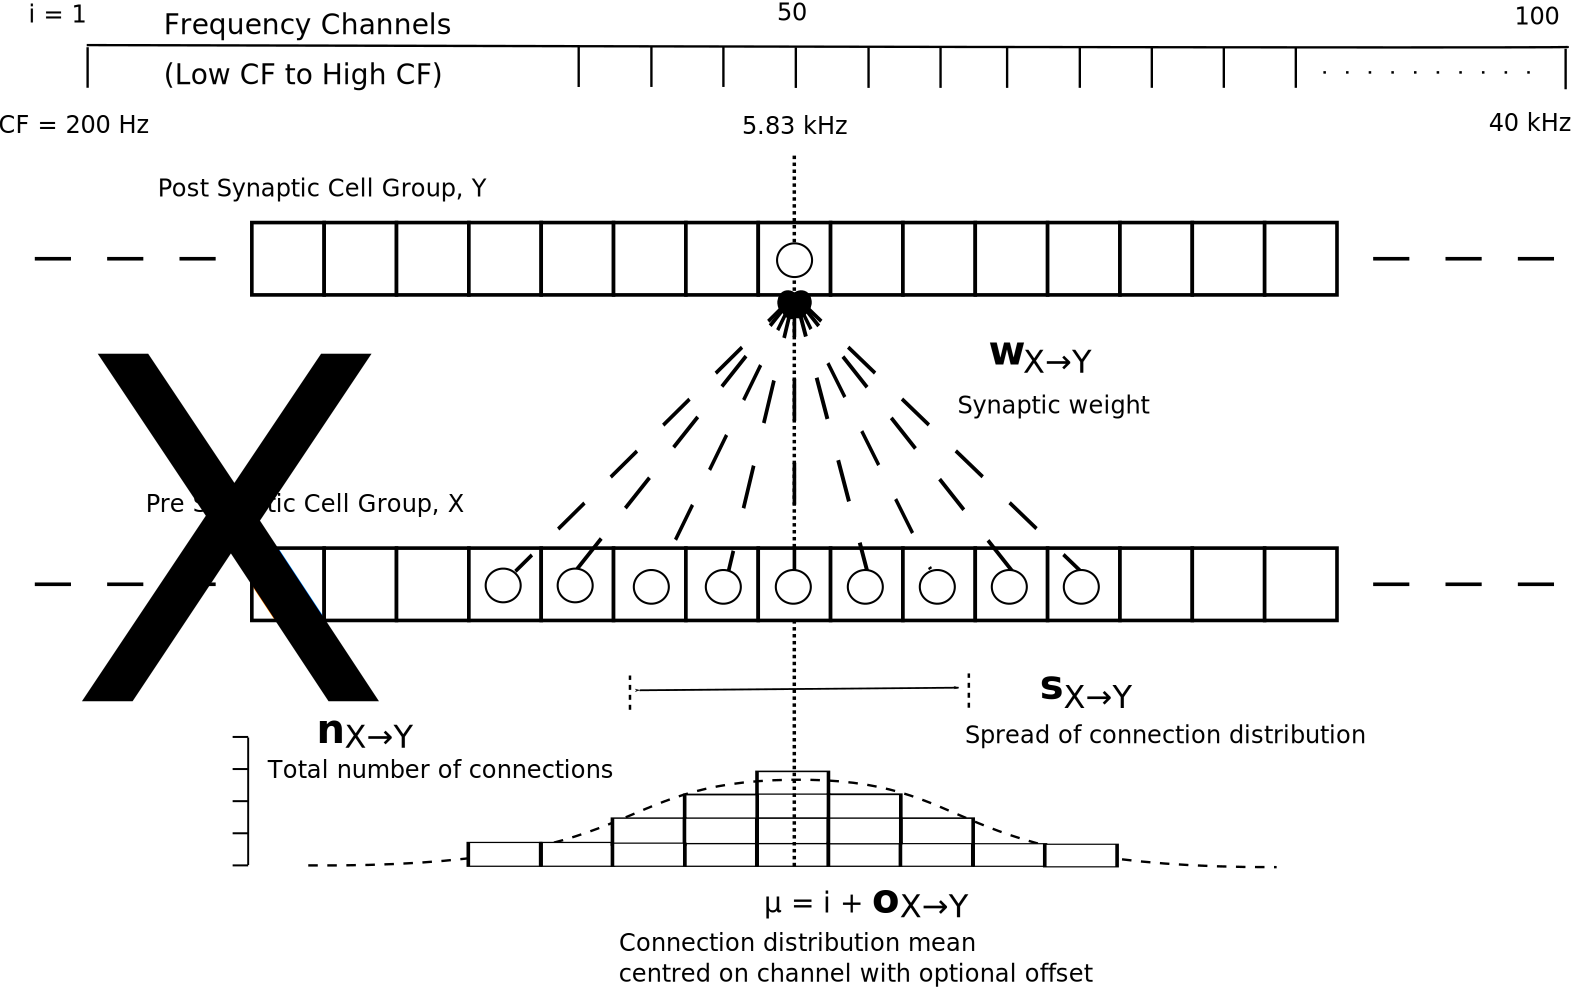
\includegraphics[keepaspectratio=true]{gfx/CNConn}}
%    \resizebox{5in}{!}{\input{./gfx/CNConn.tex}}
    \caption{Gaussian connection between cell types in cochlear
      nucleus. }
    \label{fig:CNconn}
  \end{center}
\end{figure}






%%% Local Variables: 
%%% mode: latex
%%% TeX-master: "SimpleResponses"
%%% TeX-PDF-mode: nil
%%% End: 
